\documentclass{beamer}

\mode<presentation>
{
  \usetheme{AnnArbor}
  \usecolortheme{beaver}
  %\usefonttheme{serif}
}


\usepackage[utf8]{inputenc}
\usepackage{default}
\usepackage[caption=false]{subfig}
\usepackage{graphicx}
\graphicspath{{../../Logfigures/}}
%\usepackage{pslatex}
\usepackage{setspace}
\usepackage{hyperref}
\usepackage{amssymb}
\usepackage{epstopdf}
\usepackage{listings}
\usepackage{color}
\usepackage{amsmath}
\usepackage{tikz}
\usepackage{mathtools}
\usepackage{caption}
\captionsetup[figure]{labelformat=empty}
\captionsetup{font=scriptsize,labelfont=scriptsize}
\usepackage{grffile}
\usepackage{bm}

%Equations/Entries
\newcommand{\beq}{\begin{equation}}
\newcommand{\bequo}{\begin{quotation}}
\newcommand{\beqa}{\begin{eqnarray}}
\newcommand{\eeq}{\end{equation}}
\newcommand{\leeq}[1]{\label{#1}\end{equation}}
\newcommand{\equo}{\end{quotation}}
\newcommand{\eeqa}{\end{eqnarray}}
\newcommand{\non}{\nonumber}
\newcommand{\mx}{\mbox}
\newcommand{\mxf}[1]{\mbox{\footnotesize{#1}}}
\newcommand{\lb}{\label}
\newcommand{\fr}[1]{(\ref{#1})}
\newtheorem{entry}{}[section]
\newcommand{\bent}[1]{\vspace*{-2cm}\hspace*{-1cm}\begin{entry}\lb{e{#1}}\rm}
\newcommand{\eent}{\end{entry}}
\newcommand{\fre}[1]{{\bf\ref{e{#1}}}}
\newcommand{\Emark}{$\sqcap\hspace{-2.7mm}\sqcup$}
\newcommand{\sEmark}{{\fns $\sqcap\hspace{-2.3mm}\sqcup$}}
\newcommand{\fn}{\footnote}


%Greek Letters
\renewcommand{\a}{\alpha}
\renewcommand{\b}{\beta}
\newcommand{\g}{\gamma}
\newcommand{\G}{\Gamma}
\renewcommand{\d}{\delta}
\renewcommand{\th}{\theta}
\renewcommand{\k}{\kappa}
\newcommand{\Th}{\Theta}
\newcommand{\D}{\Delta}
\newcommand{\e}{\epsilon}
\newcommand{\ep}{\varepsilon}
\newcommand{\s}{\sigma}
\renewcommand{\S}{\Sigma}
\newcommand{\w}{\omega}
\newcommand{\W}{\Omega}
\newcommand{\al}{\alpha}
\newcommand{\bet}{\beta}
\newcommand{\gam}{\gamma}
\newcommand{\lam}{\lambda}
\newcommand{\Lam}{\Lambda}
\newcommand{\eps}{\varepsilon}
\newcommand{\ichi}\sichi
\renewcommand{\ni}{\sni}
\renewcommand{\r}{\rho}
\renewcommand{\t}{\tau}
\newcommand{\ph}{\varphi}
\newcommand{\sichi}{{\mbox{{\footnotesize I}}}}
\newcommand{\sni}{{\mbox{{\footnotesize II}}}}

%color2010/6/9
\newcommand{\red}{\color{red}}
\newcommand{\blue}{\color{blue}}
\newcommand{\green}{\color{green}}
\definecolor{gray}{rgb}{0.5, 0.5, 0.5}
\newcommand{\gray}{\color{gray}}

%Derivatives
\newcommand{\pder}[2]{\frac{\partial {#1}}{\partial {#2}}}
\newcommand{\pdert}[2]{\frac{\partial^2 {#1}}{\partial {#2}^2}}
\newcommand{\fder}[2]{\frac{\delta {#1}}{\delta {#2}}}
\newcommand{\PDD}[3]{\left.\frac{\partial^{2}{#1}}{\partial{#2}^{2}}\right|_{#3}
}
\newcommand{\PD}[3]{\left.\frac{\partial{#1}}{\partial{#2}}\right|_{#3}}
\newcommand{\der}[2]{\frac{d {#1}}{d {#2}}}

\renewcommand{\deg}{^\circ}
\newcommand{\com}{{\bf [C] }}
\newcommand{\cend}{\Emark\[\]\vspace*{-1. cm}}
\newcommand{\x}{\times}

%My commands
\newcommand{\win}{\ddot\smile}
\newcommand{\lose}{\ddot\frown}
\newcommand{\avg}[1]{\left \langle #1 \right \rangle}
\newcommand{\E}[1]{\ensuremath{\times10^{#1}}}
\newcommand{\abs}[1]{\ensuremath{\left | #1 \right |}}
\newcommand{\paren}[1]{\left(#1\right)}
\newcommand{\recip}[1]{\frac{1}{#1}}
\newcommand{\ex}[1]{\mathbb{E}[#1]}
\newcommand{\bprob}[1]{\textbf{#1~---}}
\newcommand{\unitv}[1]{\ensuremath{\mathbf{\hat{e}}_{#1}}}
\newcommand{\goto}{\rightarrow}
\newcommand{\expct}[1]{\mathbb{E}[#1]}
\newcommand{\mtrx}[1]{\begin{matrix}#1\end{matrix}}
\newcommand{\pmtrx}[1]{\paren{\begin{matrix}#1\end{matrix}}}
\newcommand{\cosp}[1]{\cos{\paren{#1}}}
\newcommand{\sinp}[1]{\sin{\paren{#1}}}
\newcommand{\tanp}[1]{\tan{\paren{#1}}}
\newcommand{\half}[1]{\frac{#1}{2}}
\newcommand{\ham}{\mathcal{H}}
\newcommand{\tr}{\mathrm{Tr}}
\newcommand{\bv}[1]{\mathbf{#1}}
\newcommand{\Der}[2]{\frac{d#1}{d#2}}
\renewcommand{\Dot}[2]{\ensuremath{\bv{#1}\cdot\bv{#2}}}
\newcommand{\Cross}[2]{\ensuremath{\bv{#1}\times\bv{#2}}}
\newcommand{\del}{\ensuremath{\partial}}
\newcommand{\R}{\ensuremath{\bv{r-r'}}}
\newcommand{\aR}{\ensuremath{\abs{\R}}}
\newcommand{\br}{\ensuremath{\bv{r}}}
\newcommand{\impl}{\ensuremath{\quad \Rightarrow \quad}}
\renewcommand{\div}[1]{\nabla \cdot \bv{#1}}
\newcommand{\curl}[1]{\nabla \times \bv{#1}}
\newcommand{\lapl}{\nabla^2}
\newcommand{\vint}{\int d^3r}
\newcommand{\oocs}{\recip{c^2}}
\newcommand{\mnfp}[1]{\frac{\mu_0 #1}{4\pi}}
\renewcommand{\iiint}{\int_{-\infty}^{\infty}}
\newcommand{\tpi}[1]{\paren{2\pi}^{#1}}
\newcommand{\ootpi}[1]{\recip{\paren{2\pi}^{#1}}}


\title{Phonons, Librons, and Topological Defects}
\author{Jim Antonaglia}
\date{February 12, 2015}
\begin{document}
%%%%% 1 %%%%%
\frame{
\maketitle
}

%% Phonon and libron stuff %%
\frame{
\frametitle{Work in the literature}
\begin{itemize}
\item J.C. Raich and R.D. Etters, \emph{J. Chem. Phys.}, \textbf{55} 8 (1971): ``Soft Modes in Molecular Crystals." Used the ``self-consistent phonon approximation" in a linear chain of dumbbells and other systems and found libron modes that weren't gapped. Explicitly makes the assumption that $V(\th_i,\th_j) = V(\th_i-\th_j)$, which removes the libron band gap by hand.
\item B, Kamgar-Parsi, E. G. D. Cohen, and I.M. de Schepper, \emph{Phys. Rev. A}, \textbf{35} 11 (1987): ``Dynamical processes in hard-sphere fluids." Explicitly treats the hard-sphere interactions and defines regimes of packing fraction and wavenumber where hydrodynamical modes are well-defined. Totally over my head in terms of jargon, and figures and results are unintuitive. Enskog operator? BKG approximation?
\end{itemize}
}

\frame{
\begin{itemize}
\frametitle{Work in the literature}
\item Taner Yildirim, \emph{Solid State Communications}, 124 (2002) 449--455: ``Lattice dynamics of solid cubans within the quasi-harmonic approximation." Uses empirically determined interatomic potentials for cubane (C$_8$H$_8$) molecules and makes an enormous dynamical matrix out of the quadratic approximations to the pair potentials. Doesn't treat the non-commutativity of 3D rotations at all, finds phonons and librons are weakly coupled, \emph{does} find that they are gapped.
\item P. Keim, G. Maret, U. Herz, and H.H. von Grunberg, \emph{Phys. Rev. Lett.} \textbf{92} 21 (2004): ``Harmonic Lattice Behavior of Two-Dimensional Colloidal Crystals." Experimental work: takes microvideography of 2D spherical colloids and uses correlation functions to determine the phonon mode frequencies of colloids interacting with $1/r^3$ repulsive potentials. ``Our results demonstrate that a colloidal crystal can be seen as a bead-spring lattice immersed in a viscous fluid. A normal vibration mode then transforms into a `normal relaxation mode.'"
\end{itemize}
}

\frame{
\frametitle{Work in the literature}
\begin{itemize}
\item Can't find papers treating librons outside the context of molecular crystals. Modes do not appear in hard particle systems unless they're hard spheres, in which the libron doesn't exist.
\end{itemize}
}

%% Phonon and libron %%
\frame{
\begin{center}
Phonons and Librons in Hard Hexagons
\end{center}
}

%%%%%%
\frame{
\begin{figure}
\centering
\includegraphics[scale=0.45]{{N=[2500]_pfi=[0.8, 0.79, 0.78, 0.77, 0.76, 0.75, 0.74, 0.73, 0.72, 0.715, 0.71]_steps=[10000000.0]_yy_kx=0}.pdf}
\caption{Longitudinal phonon for $N=50^2$ and $s=10^7$ and for $\phi$ decreasing from $0.800$ to $0.710$. The first major jump occurs between $0.730$ and $0.720$, then another one from $0.720$ to $0.715$. Note also that the theoretical curves fail to fit the phonon dispersion for large $\abs{\bv k}$ at higher densities.}
\end{figure}
}

\frame{
\begin{figure}
\centering
\includegraphics[scale=0.45]{{N=[2500]_pfi=[0.8, 0.79, 0.78, 0.77, 0.76, 0.75, 0.74, 0.73, 0.72, 0.715, 0.71]_steps=[10000000.0]_thth_kx=0}.pdf}
\caption{Libron for $N=50^2$ and $s=10^7$ and for $\phi$ decreasing from $0.800$ to $0.710$. The libron dispersion is more or less smooth as the density is decreased, unlike the phonon dispersion.}
\end{figure}
}

\frame{
\begin{figure}
\centering
\includegraphics[scale=0.45]{{N=[2500]_pfi=[0.71, 0.709, 0.708, 0.707, 0.706, 0.705, 0.704, 0.703, 0.702, 0.701, 0.7]_steps=[10000000.0]_thth_kx=0}.pdf}
\caption{Libron for $N=50^2$ and $s=10^7$ and for $\phi$ decreasing from $0.710$ to $0.700$. The libron dispersion deviates more and more from predicted theory curves as the density is decreased. Large $k$ dispersion is relatively flat near $\phi = 0.700$ and the $\bv k = 0$ mode frequency decreases with decreasing density.}
\end{figure}
}

\frame{
\begin{figure}
\centering
\includegraphics[scale=0.45]{{N=[10000]_pfi=[0.8, 0.75, 0.71]_steps=[10000000.0]_yy_kx=0}.pdf}
\caption{Longitudinal phonon for $N=100^2$ and $s=10^7$ and for $\phi$ decreasing from $0.800$ to $0.710$. The same features are present, a jump to a near flat dispersion around $\phi = 0.710$. Figure \ref{phi6} shows lower $\phi$ with a smaller $y$-axis.}
\end{figure}
}

\frame{
\begin{figure}
\centering
\includegraphics[scale=0.45]{{N=[10000]_pfi=[0.71, 0.7, 0.69, 0.68]_steps=[10000000.0]_yy_kx=0}.pdf}
\caption{Longitudinal phonon for $N=100^2$ and $s=10^7$ and for $\phi$ decreasing from $0.710$ to $0.680$. Zooming in reveals that the dispersion curves don't fit the theory at all near the phase transition (to be expected), and error bars are very large compared to the magnitude of the dispersion itself.}
\label{phi6}
\end{figure}
}

\frame{
\begin{figure}
\centering
\includegraphics[scale=0.45]{{N=[10000]_pfi=[0.8, 0.75, 0.71, 0.7, 0.69, 0.68]_steps=[10000000.0]_thth_kx=0}.pdf}
\caption{Libron dispersion for $N=100^2$ and $s=10^7$. As the density is lowered closer to the hexatic$\goto$ fluid transition, the libron's dispersion becomes flatter for $k>0$ and the $\bv k = 0$ mode $\goto$ 0. Once $\w(\bv k = 0) = 0$, this signifies a density at which the libron mode is no longer massive and a uniform rotation of the hexagons no longer costs energy (or rather entropy).}
\label{phi7}
\end{figure}
}

\frame{
\begin{figure}
\centering
\includegraphics[scale=0.45]{{N=[10000]_pfi=[0.7, 0.69, 0.68]_steps=[10000000.0]_thth_kx=0}.pdf}
\caption{Libron dispersion for $N=100^2$ and $s=10^7$ but only for lower densities. It may not be clear, but the error bars near $k = 0$ are actually very small, compared to the error bars at $k>0$.}
\label{phi8}
\end{figure}
}

\frame{

Near phase transitions, the phonon and libron spectra become flat except for at $\bv k = 0$. I'd like to explore what that signifies. The potential energy part of the Hamiltonian expressed in terms of the Fourier components of the libron field $\tilde \th_{\bv k}$ (I'll just use the libron field for simplicity, and without loss of generality, because the librons and phonons are uncoupled at these densities anyway) is
\beq \mathcal{H} = \half{1} \sum_{\bv k} \tilde \th^*_{\bv k} K_{\th\th,\bv k} \tilde \th_{\bv k}. \eeq
If we let $K_{\th\th,\bv k=0} = 0$ and $K_{\th\th}$ for all other $\bv k$ vectors. So let's put that in:
\beq \mathcal{H} = \half{1}K_{\th\th} \sum_{\bv k \neq 0} \tilde \th^*_{\bv k} \tilde \th_{\bv k} + \half{1}K_{\th\th}\e = \half{1}K_{\th\th} \sum_{\bv k} \tilde \th^*_{\bv k} \tilde \th_{\bv k} - \half{1}K_{\th\th}(1-\e) \tilde \th^*_{0} \tilde \th_{0}. \eeq
Performing the inverse Fourier transform:
\beq \mathcal{H} = \half{1}K_{\th\th} \sum_{i} \th_i^2 - \recip{2N} K_{\th\th}(1-\e) \sum_{i,j} \th_i \th_j. \eeq
\beq \mathcal{H} = \recip{2N} K_{\th\th} \bm \th \cdot \pmtrx{N-1 & -1 & -1 & -1 & \ldots \\ -1 & N-1 & -1 & -1 & -1 \\ -1 & -1 & N-1 & -1 & -1 \\ -1 & -1 & -1 & N-1 & -1 \\ \vdots & -1 & -1 & -1 & \ddots} \cdot \bm \th = \half{1} \th_i K'_{ij} \th_j \eeq
The determinant of the matrix $\bv K'$ is zero. $\bv K'$ no longer has an inverse and correlation functions will no longer be well defined. The $\bv k = 0$ mode is \emph{floppy}. However, if we examine the components of $K'_{ij}$, all the off-diagonal components are nonzero and of order $1/N$, whereas the diagonal components are of order $1$. There is \emph{nonzero coupling to every particle in the system} but there is \emph{no cost to rotating all the particles the same amount}. That is, we can send every $\th_i \goto \th_i + \Delta \th$ and it wouldn't cost any energy. However, \emph{every particle is weakly coupled to every other particle}, and by weakly, it is meant that the coupling between $\th_i$ and $\th_j$ is order $1/N$ (but there are $\sim N$ degrees of freedom that $\th_i$ is coupled to, so it is weakly coupled to the whole system by $\mathcal{O}(1)$ interactions). The way I am interpreting this is that this represents an ideal gas that is coupled in a mean-field manner to itself, just like the infinite-range Ising model.

}


%% Topological defect stuff %%

\frame{
\begin{center}
Topological Defects
\end{center}
}

%%  %%
\frame{
\frametitle{$\phi=0.710$, $N=50^2$}
\begin{figure}
\centering
 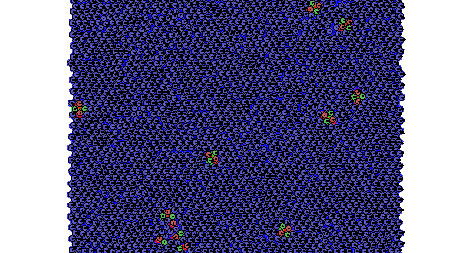
\includegraphics[scale=1.4]{phi071_bounddislocations.pdf}
\end{figure}
$\phi = 0.710$, a few dislocation/anti-dislocation pairs. One dislocation 
triplet. Unbinding is extremely unfavorable.
}

%%  %%
\frame{ 
\frametitle{$\phi=0.700$, clustering, dislocation unbinding}
\begin{figure}
 \centering
 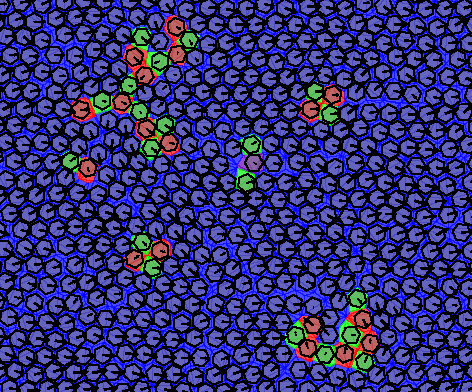
\includegraphics[scale=1.1]{phi070_stringofdefects.pdf}
\end{figure}
}

%%  %%
\frame{ 
\frametitle{$\phi=0.685$, hexatic domain walls}
\begin{figure}
 \centering
 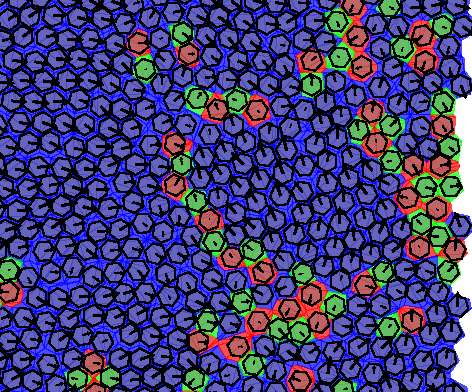
\includegraphics[scale=1.1]{phi0685_boundaries.pdf}
\end{figure}
}

%%  %%
\frame{ 
\frametitle{$\phi=0.685$, well in the hexatic phase}
\begin{figure}
 \centering
 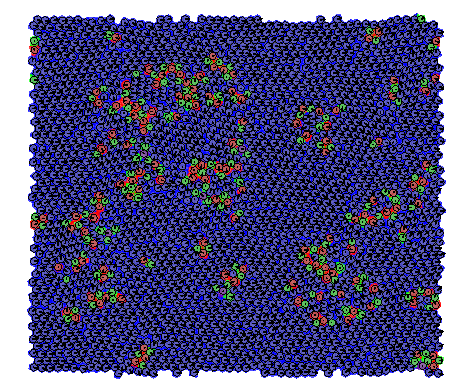
\includegraphics[scale=1.2]{phi0685_hexaticphase.pdf}
\end{figure}
}

%%  %%
\frame{
\frametitle{$\phi=0.680$, disclination unbinding}
\begin{figure}
 \centering
 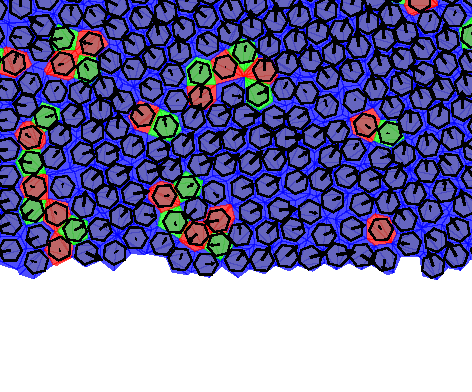
\includegraphics[scale=1.2]{phi068_antivortex.pdf}
\end{figure}
}

%%  %%
\frame{
\frametitle{$\phi=0.680$, disclination unbinding}
\begin{figure}
 \centering
 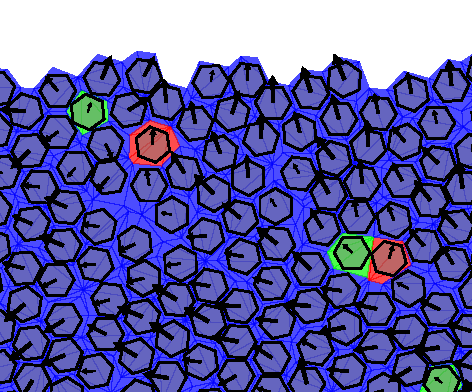
\includegraphics[scale=1.2]{phi068_vortexpairs.pdf}
\end{figure}
}

%%  %%
\frame{
\frametitle{$\phi=0.680$, disclination unbinding}
\begin{figure}
 \centering
 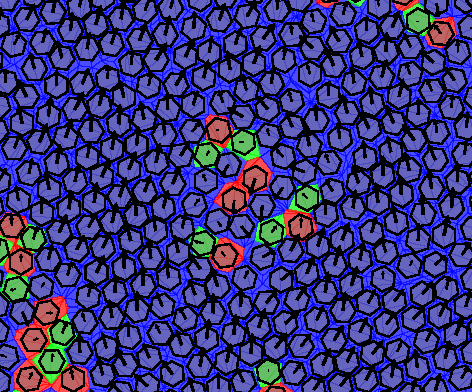
\includegraphics[scale=1.2]{phi068_netvortices.pdf}
\end{figure}
}

%%  %%
\frame{ 
\frametitle{$\phi=0.670$, $N=128^2$}
\begin{figure}
 \centering
 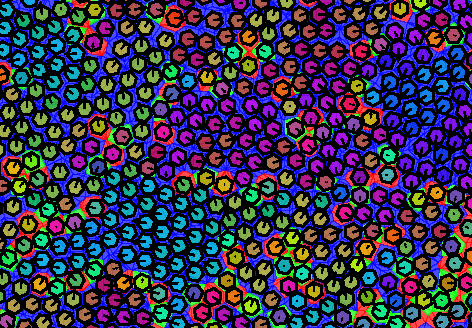
\includegraphics[scale=1.35]{phi067_N16000_color.pdf}
\end{figure}
}

%%  %%
\frame{
\frametitle{Phonon/libron modes: defects affect stiffness 
constants}
Light blue: phonon elastic stiffness. Red: libron elastic stiffness. Blue: 
libron mass. Green: libron-phonon coupling (0 by symmetry).
\begin{figure}
\captionsetup[subfigure]{labelformat=empty}
 \subfloat[$\phi$]{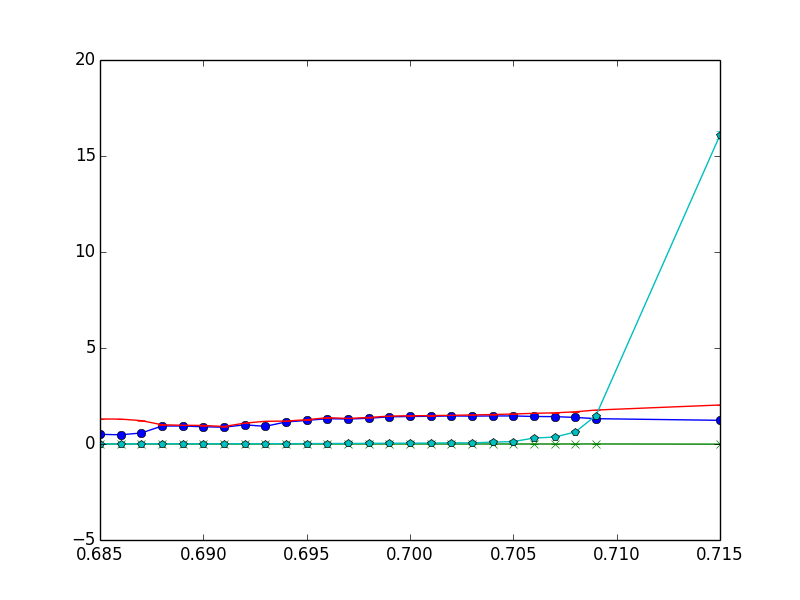
\includegraphics[scale=0.3]{couplings_zoom.png} }
 \subfloat[$\phi$]{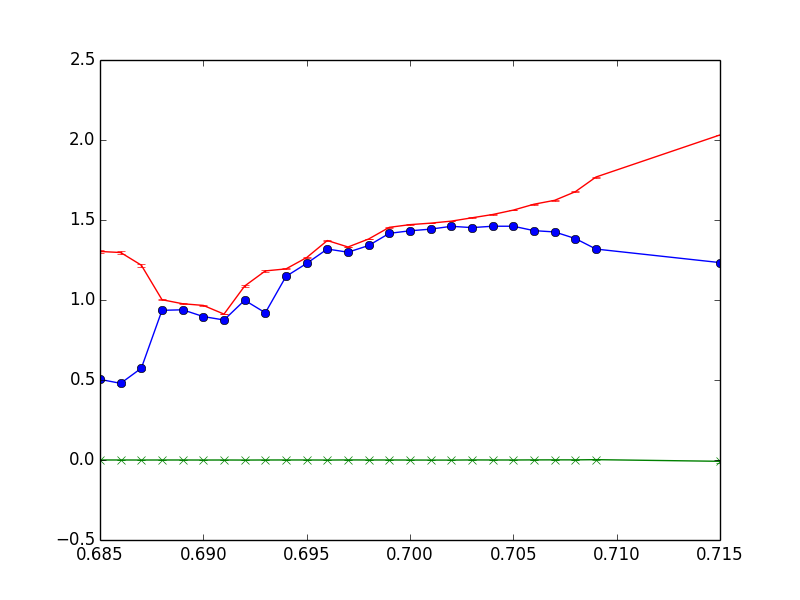
\includegraphics[scale=0.3]{libcouplings_zoom.png} }
\end{figure}
}



\end{document}